\documentclass[]{article}
\usepackage{lmodern}
\usepackage{amssymb,amsmath}
\usepackage{ifxetex,ifluatex}
\usepackage{fixltx2e} % provides \textsubscript
\ifnum 0\ifxetex 1\fi\ifluatex 1\fi=0 % if pdftex
  \usepackage[T1]{fontenc}
  \usepackage[utf8]{inputenc}
\else % if luatex or xelatex
  \ifxetex
    \usepackage{mathspec}
  \else
    \usepackage{fontspec}
  \fi
  \defaultfontfeatures{Ligatures=TeX,Scale=MatchLowercase}
\fi
% use upquote if available, for straight quotes in verbatim environments
\IfFileExists{upquote.sty}{\usepackage{upquote}}{}
% use microtype if available
\IfFileExists{microtype.sty}{%
\usepackage{microtype}
\UseMicrotypeSet[protrusion]{basicmath} % disable protrusion for tt fonts
}{}
\usepackage[margin=1in]{geometry}
\usepackage{hyperref}
\hypersetup{unicode=true,
            pdftitle={IPA Small and Mid cap analysis},
            pdfauthor={Søren Schwartz},
            pdfborder={0 0 0},
            breaklinks=true}
\urlstyle{same}  % don't use monospace font for urls
\usepackage{graphicx,grffile}
\makeatletter
\def\maxwidth{\ifdim\Gin@nat@width>\linewidth\linewidth\else\Gin@nat@width\fi}
\def\maxheight{\ifdim\Gin@nat@height>\textheight\textheight\else\Gin@nat@height\fi}
\makeatother
% Scale images if necessary, so that they will not overflow the page
% margins by default, and it is still possible to overwrite the defaults
% using explicit options in \includegraphics[width, height, ...]{}
\setkeys{Gin}{width=\maxwidth,height=\maxheight,keepaspectratio}
\IfFileExists{parskip.sty}{%
\usepackage{parskip}
}{% else
\setlength{\parindent}{0pt}
\setlength{\parskip}{6pt plus 2pt minus 1pt}
}
\setlength{\emergencystretch}{3em}  % prevent overfull lines
\providecommand{\tightlist}{%
  \setlength{\itemsep}{0pt}\setlength{\parskip}{0pt}}
\setcounter{secnumdepth}{0}
% Redefines (sub)paragraphs to behave more like sections
\ifx\paragraph\undefined\else
\let\oldparagraph\paragraph
\renewcommand{\paragraph}[1]{\oldparagraph{#1}\mbox{}}
\fi
\ifx\subparagraph\undefined\else
\let\oldsubparagraph\subparagraph
\renewcommand{\subparagraph}[1]{\oldsubparagraph{#1}\mbox{}}
\fi

%%% Use protect on footnotes to avoid problems with footnotes in titles
\let\rmarkdownfootnote\footnote%
\def\footnote{\protect\rmarkdownfootnote}

%%% Change title format to be more compact
\usepackage{titling}

% Create subtitle command for use in maketitle
\newcommand{\subtitle}[1]{
  \posttitle{
    \begin{center}\large#1\end{center}
    }
}

\setlength{\droptitle}{-2em}

  \title{IPA Small and Mid cap analysis}
    \pretitle{\vspace{\droptitle}\centering\huge}
  \posttitle{\par}
    \author{Søren Schwartz}
    \preauthor{\centering\large\emph}
  \postauthor{\par}
      \predate{\centering\large\emph}
  \postdate{\par}
    \date{22 sep 2018}

\usepackage{booktabs}
\usepackage{longtable}
\usepackage{array}
\usepackage{multirow}
\usepackage[table]{xcolor}
\usepackage{wrapfig}
\usepackage{float}
\usepackage{colortbl}
\usepackage{pdflscape}
\usepackage{tabu}
\usepackage{threeparttable}
\usepackage{threeparttablex}
\usepackage[normalem]{ulem}
\usepackage{makecell}

\usepackage{float}

\begin{document}
\maketitle

\hypertarget{indledning}{%
\section{Indledning}\label{indledning}}

Analysen er lavet for at undersøge om man ved en relativ momentum
strategi kan opnå profit på det danske small og mid cap marked. I første
omgang ses på momentum i forskellige tidsperioder, og senere tages højde
for transaktionsomkostninger. I den forbindelse er det klart, at handles
der ofte med få aktiver pr. handel, da bliver den relative omkostning
pr. aktiv stor. Der forsøges derfor også at se på, om man ved at ændre
på mængden af aktier handlet pr. gang kan ændrer
transaktionsomkostningernes betydning. Det er antaget at
transaktionskostninger er 0.01 \% ved et minimum beløb på 29 kr. Til
sidst prøves en ``Error adjusted'' relativ momentum strategi for at se
om man kan implementere en strategi der nedjusterer antallet af handler,
og er mere robust overfor støj.

Small og Mid cap gruppering er fundet fra
\href{https://www.euroinvestor.dk/markeder/aktier/europa/danmark}{Euroinvestor}.
Gruppen af Mid cap består af 25 aktiver, hvor gruppen af Small cap
består af 71 (i disse tal er fratrukket de aktiver, som ikke tages med i
analysen).

Aktiver hvor data ikke kan fås fra
\href{https://finance.yahoo.com/}{Yahoo Finance} fra start 2017 eller de
ikke handles på den Københavnske børs er ikke taget med. Dette er:

\begin{itemize}
\tightlist
\item
  InterMail B A/S
\item
  German High Street Properties
\item
  Athena Investments
\end{itemize}

\hypertarget{trend-i-forskellige-tidsperiod}{%
\section{Trend i forskellige
tidsperiod}\label{trend-i-forskellige-tidsperiod}}

I dette afsnit ses på relativ momentum uden transaktionsmkostninger,
hvor man hele tiden har en position i de 15 aktiver, som strategien
giver klarer sig bedst.

Strategien består i at finde ROC \emph{(Rate of Change)} for perioderne
3, 6, 12 måneder. Dertil findes også en ROC som gennemsnit af disse
\emph{(Ave)}, og en ROC med mere vægt på 6 måneders afkast
\emph{(Weighted Ave)}. Ud fra disse laves en rangering af de bedste
aktiver, hvor det i dette afsnit er de 15 bedste.

\begin{figure}
\centering
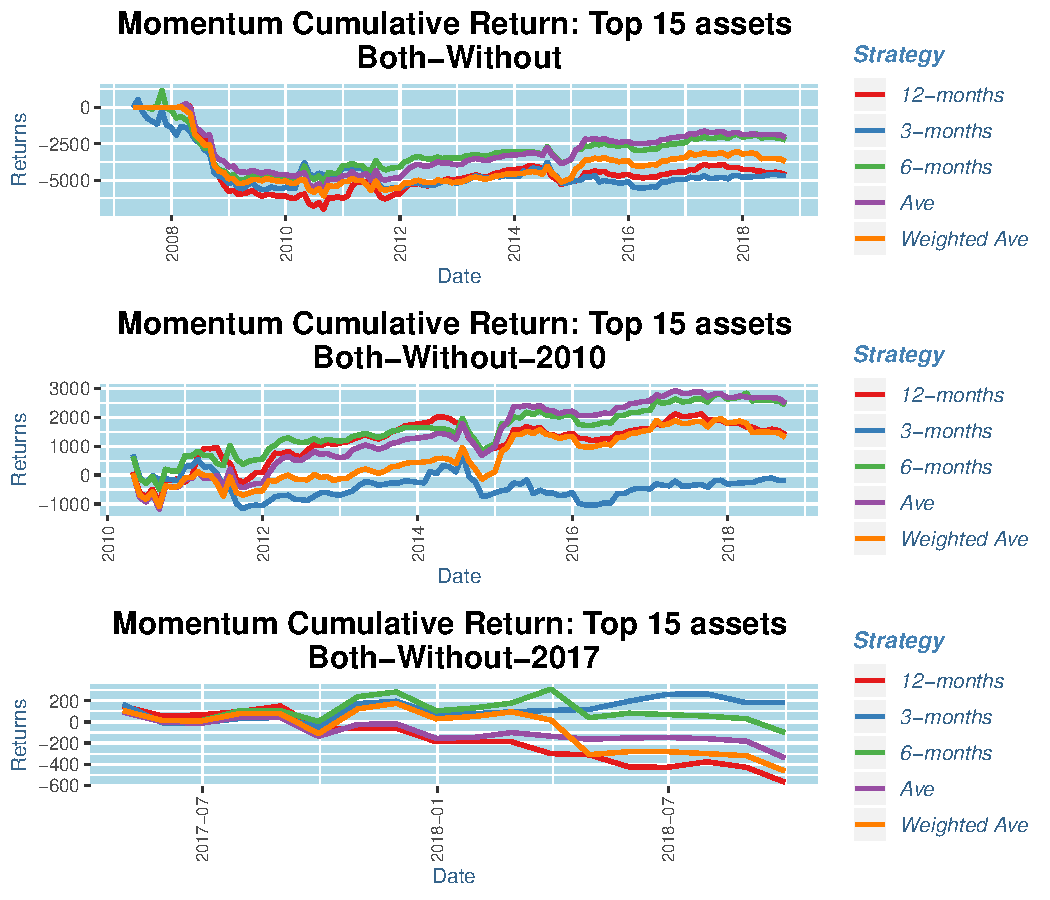
\includegraphics{IPA_Small_and_Mid_files/figure-latex/fig4-1.pdf}
\caption{\label{fig:withOut}Top 15 aktiver for portefølje af både Small-
og Mid cap uden transaktions omkostninger med månedlig rebalancering}
\end{figure}

\rowcolors{2}{gray!6}{white}
\begin{table}

\caption{\label{tab:tab4}\label{tab:withOut}Top 15 aktiver for månedlig rebalancering for portefølje af både Small- og Mid cap uden transaktionsomkostninger}
\centering
\resizebox{\linewidth}{!}{
\begin{tabular}[t]{lrrrrrrrrrrrrrrr}
\hiderowcolors
\toprule
\multicolumn{1}{c}{} & \multicolumn{5}{c}{2007-2018} & \multicolumn{5}{c}{2010-2018} & \multicolumn{5}{c}{2017-2018} \\
\cmidrule(l{2pt}r{2pt}){2-6} \cmidrule(l{2pt}r{2pt}){7-11} \cmidrule(l{2pt}r{2pt}){12-16}
  & 3-months & 6-months & 12-months & Ave & Weighted Ave & 3-months & 6-months & 12-months & Ave & Weighted Ave & 3-months & 6-months & 12-months & Ave & Weighted Ave\\
\midrule
\showrowcolors
Observations & 138.0000 & 138.0000 & 138.0000 & 138.0000 & 138.0000 & 102.0000 & 102.0000 & 102.0000 & 102.0000 & 102.0000 & 18.0000 & 18.0000 & 18.0000 & 18.0000 & 18.0000\\
NAs & 3.0000 & 3.0000 & 3.0000 & 3.0000 & 3.0000 & 3.0000 & 3.0000 & 3.0000 & 3.0000 & 3.0000 & 3.0000 & 3.0000 & 3.0000 & 3.0000 & 3.0000\\
Minimum & -1378.3543 & -1229.4482 & -1657.1882 & -1351.2780 & -1449.7623 & -777.4320 & -745.7288 & -699.4882 & -825.0409 & -734.5911 & -174.9746 & -270.9071 & -212.1087 & -179.3584 & -326.1903\\
Quartile 1 & -119.0684 & -95.7579 & -94.0674 & -77.8627 & -85.7132 & -51.8966 & -63.6464 & -63.4786 & -49.0416 & -79.2429 & -0.0047 & -79.2676 & -107.7502 & -33.1497 & -90.8533\\
Median & -7.7173 & 0.1666 & 0.1863 & 1.1733 & 0.0000 & 7.9686 & 6.5246 & 11.6353 & 12.4510 & 16.8837 & 10.6629 & -1.2048 & -5.8671 & -6.8991 & -3.7510\\
\addlinespace
Arithmetic Mean & -33.9417 & -16.2334 & -33.6212 & -14.8974 & -26.7327 & -1.8849 & 23.7883 & 13.7063 & 24.4782 & 12.8626 & 10.0886 & -5.5646 & -31.7056 & -18.8965 & -25.7886\\
Geometric Mean & NaN & NaN & NaN & NaN & NaN & NaN & NaN & NaN & NaN & NaN & NaN & NaN & NaN & NaN & NaN\\
Quartile 3 & 79.3906 & 94.0700 & 78.3190 & 77.1780 & 70.1526 & 79.3906 & 96.7741 & 88.1401 & 96.9755 & 86.8658 & 36.8567 & 44.6488 & 10.4532 & 11.2884 & 38.9583\\
Maximum & 1091.7807 & 1019.1891 & 793.3409 & 788.6953 & 716.4210 & 701.3248 & 699.7260 & 793.3409 & 788.6953 & 716.4210 & 223.0438 & 235.3860 & 149.5407 & 113.0603 & 234.6610\\
SE Mean & 26.1758 & 24.4472 & 23.9826 & 22.6026 & 23.1214 & 21.4029 & 22.4190 & 20.4690 & 22.3600 & 22.1674 & 22.2602 & 28.1875 & 20.5977 & 18.7976 & 29.4608\\
\addlinespace
LCL Mean (0.95) & -85.7026 & -64.5760 & -81.0452 & -59.5924 & -72.4536 & -44.3424 & -20.6849 & -26.8987 & -19.8781 & -31.1116 & -36.8763 & -65.0350 & -75.1630 & -58.5560 & -87.9455\\
UCL Mean (0.95) & 17.8191 & 32.1093 & 13.8027 & 29.7976 & 18.9883 & 40.5726 & 68.2615 & 54.3114 & 68.8344 & 56.8369 & 57.0535 & 53.9058 & 11.7518 & 20.7630 & 36.3683\\
Variance & 94553.8520 & 82477.7676 & 79372.8857 & 70500.8113 & 73774.5435 & 46724.4064 & 51266.1950 & 42736.0073 & 50997.0185 & 50122.3301 & 8919.2966 & 14301.6253 & 7636.7919 & 6360.3155 & 15622.9206\\
Stdev & 307.4961 & 287.1894 & 281.7319 & 265.5199 & 271.6147 & 216.1583 & 226.4204 & 206.7269 & 225.8252 & 223.8802 & 94.4420 & 119.5894 & 87.3887 & 79.7516 & 124.9917\\
Skewness & -0.4510 & -0.6474 & -2.2501 & -1.6592 & -1.8488 & -0.5654 & 0.4182 & 0.0153 & 0.0110 & 0.1454 & 0.2175 & -0.2827 & -0.1602 & -0.5217 & -0.4082\\
\addlinespace
Kurtosis & 4.5070 & 5.0669 & 10.9091 & 8.9626 & 9.8679 & 3.8457 & 2.8215 & 4.0581 & 3.6828 & 2.6874 & 0.4591 & 0.1328 & -0.2268 & -0.2699 & 0.6649\\
NumberOfTrades & 1801.0000 & 1189.0000 & 829.0000 & 1043.0000 & 1027.0000 & 1334.0000 & 908.0000 & 638.0000 & 802.0000 & 798.0000 & 222.0000 & 156.0000 & 100.0000 & 134.0000 & 144.0000\\
\bottomrule
\end{tabular}}
\end{table}
\rowcolors{2}{white}{white}

I figur \ref{fig:withOut} kan man se momentum over forskellige perioder.
Det er tydeligt at se, at momentum er meget overhængigt af over hvilken
periode man kigger over. I krisen rundt 2008 klarer samtlige aktiver sig
dårligt og i perioden fra 2017 til i dag giver strategien ikke noget
afkast. Derfor ved at implementere handelsomkostninger i disse perioder
er det klart, at tabet blot vil være endnu større. Tabel
\ref{tab:withOut} giver relevante værdier for strategierne.

\hypertarget{trend-fordelt-pa-small--og-mid-cap}{%
\section{Trend fordelt på Small- og Mid
cap}\label{trend-fordelt-pa-small--og-mid-cap}}

I dette afsnit forsøger at kigge på perioderne 2010 til i dag og 2017
til i dag opdelt på Small- og Mid cap. Der er fortsat ingen
handelsomkostninger. Da grupperne er mindre tages nu kun top 10 med for
begge grupper \emph{(man kunne have taget procent af gruppen, hvilket er
undersøgt med samme resultat)}.

\begin{figure}
\centering
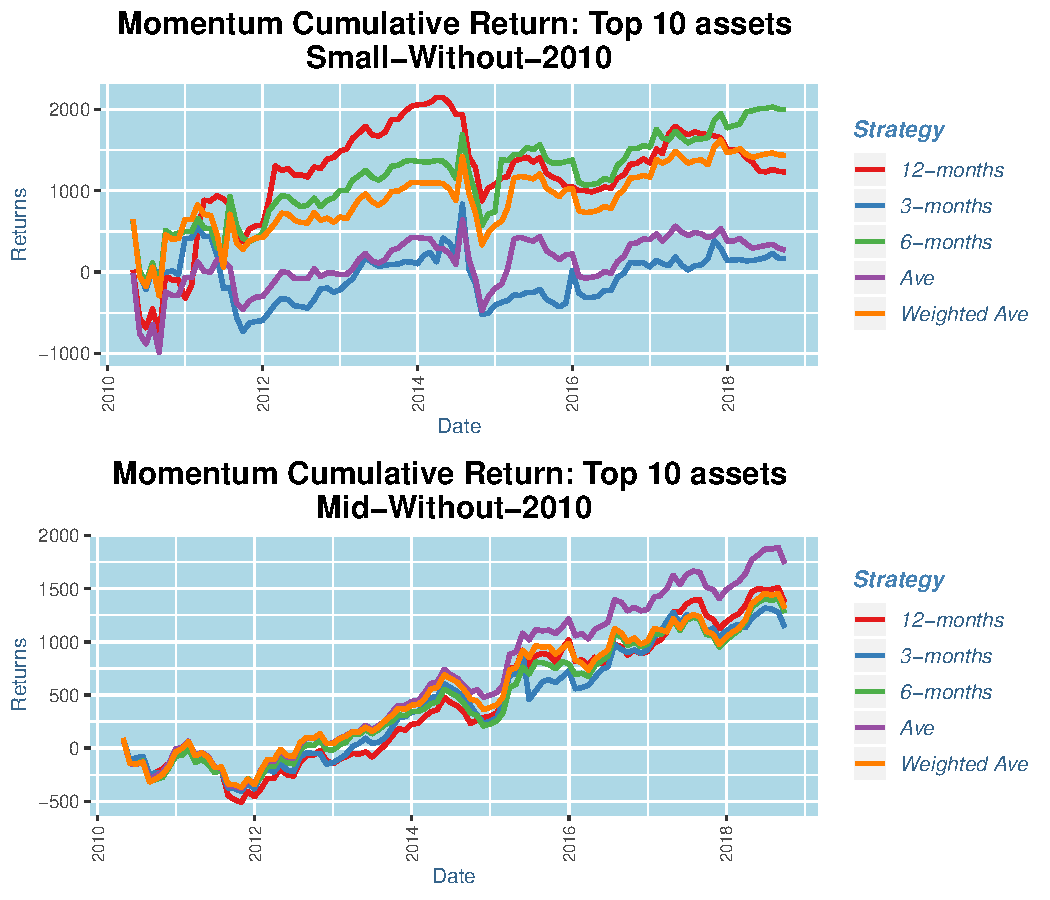
\includegraphics{IPA_Small_and_Mid_files/figure-latex/fig1-1.pdf}
\caption{\label{fig:OpdeltwithOut2010}Top 15 aktiver for Small- og Mid
cap uden transaktionsomkostninger med månedlig rebalancering fra 2010}
\end{figure}

\rowcolors{2}{gray!6}{white}
\begin{table}

\caption{\label{tab:tab1}\label{tab:OpdeltwithOut2010}Top 15 aktiver for Small- og Mid cap uden transaktionsomkostninger med månedlig rebalancering fra 2010}
\centering
\resizebox{\linewidth}{!}{
\begin{tabular}[t]{lrrrrrrrrrr}
\hiderowcolors
\toprule
\multicolumn{1}{c}{} & \multicolumn{5}{c}{2010-2018} & \multicolumn{5}{c}{2017-2018} \\
\cmidrule(l{2pt}r{2pt}){2-6} \cmidrule(l{2pt}r{2pt}){7-11}
  & 3-months & 6-months & 12-months & Ave & Weighted Ave & 3-months & 6-months & 12-months & Ave & Weighted Ave\\
\midrule
\showrowcolors
Observations & 102.0000 & 102.0000 & 102.0000 & 102.0000 & 102.0000 & 102.0000 & 102.0000 & 102.0000 & 102.0000 & 102.0000\\
NAs & 3.0000 & 3.0000 & 3.0000 & 3.0000 & 3.0000 & 3.0000 & 3.0000 & 3.0000 & 3.0000 & 3.0000\\
Minimum & -808.1948 & -597.5343 & -588.3113 & -738.8115 & -703.1205 & -442.9008 & -233.3002 & -237.0438 & -233.3002 & -233.3002\\
Quartile 1 & -52.4994 & -36.8195 & -50.8430 & -48.9638 & -51.1700 & -30.5586 & -27.1496 & -32.8506 & -23.3303 & -32.8222\\
Median & 7.9142 & 15.0269 & 2.7624 & 3.2063 & 6.5794 & 20.6497 & 22.3686 & 23.1828 & 23.0935 & 21.7422\\
\addlinespace
Arithmetic Mean & 1.6316 & 19.6164 & 12.0742 & 2.6419 & 14.0825 & 11.1550 & 12.5064 & 13.4574 & 17.0527 & 12.9138\\
Geometric Mean & NaN & NaN & NaN & NaN & NaN & NaN & NaN & NaN & NaN & NaN\\
Quartile 3 & 63.5826 & 68.0663 & 66.3393 & 64.6698 & 79.4204 & 62.9767 & 51.9513 & 60.6278 & 67.5835 & 51.9309\\
Maximum & 635.7702 & 722.8318 & 747.2986 & 746.0661 & 751.7787 & 251.7226 & 248.0253 & 286.0822 & 291.4989 & 257.8194\\
SE Mean & 18.4836 & 19.3866 & 17.3916 & 17.1171 & 19.6505 & 9.1254 & 7.6879 & 8.5270 & 8.1006 & 8.1544\\
\addlinespace
LCL Mean (0.95) & -35.0348 & -18.8414 & -22.4259 & -31.3138 & -24.8988 & -6.9473 & -2.7443 & -3.4579 & 0.9833 & -3.2623\\
UCL Mean (0.95) & 38.2980 & 58.0742 & 46.5744 & 36.5975 & 53.0638 & 29.2574 & 27.7572 & 30.3726 & 33.1221 & 29.0899\\
Variance & 34847.4627 & 38335.7303 & 30851.5841 & 29885.4144 & 39386.5785 & 8493.8192 & 6028.5838 & 7416.3835 & 6693.1761 & 6782.3780\\
Stdev & 186.6748 & 195.7951 & 175.6462 & 172.8740 & 198.4605 & 92.1619 & 77.6440 & 86.1184 & 81.8118 & 82.3552\\
Skewness & -0.5106 & 0.8408 & 0.5307 & -0.1792 & 0.4773 & -1.2061 & -0.2312 & -0.2693 & -0.1424 & -0.2066\\
\addlinespace
Kurtosis & 5.9946 & 4.2511 & 5.5408 & 6.8018 & 4.4872 & 5.0188 & 1.0087 & 1.1824 & 1.2506 & 0.6819\\
NumberOfTrades & 932.0000 & 654.0000 & 416.0000 & 536.0000 & 552.0000 & 550.0000 & 352.0000 & 248.0000 & 274.0000 & 302.0000\\
\bottomrule
\end{tabular}}
\end{table}
\rowcolors{2}{white}{white}

Fra 2010 til i dag klarer begge grupper sig godt, hvilket ses i figur
\ref{fig:OpdeltwithOut2010} og tabel \ref{tab:OpdeltwithOut2010}.

\begin{figure}
\centering
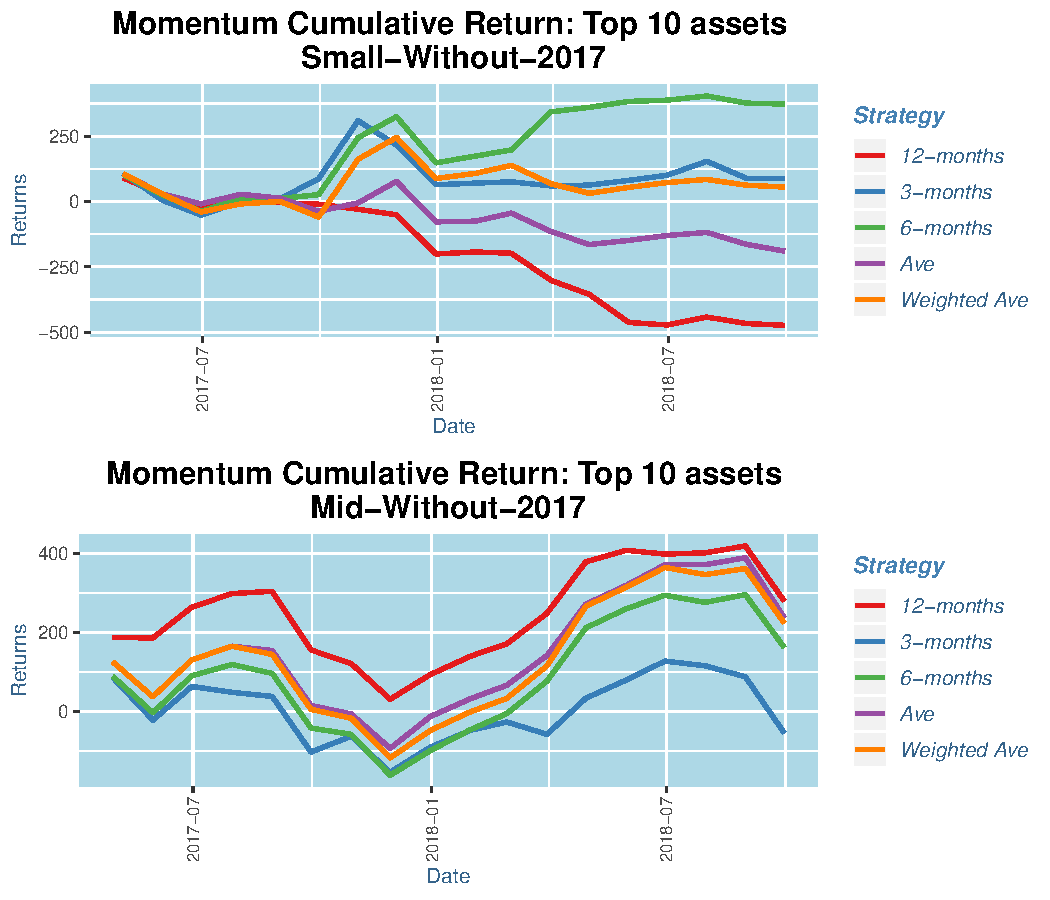
\includegraphics{IPA_Small_and_Mid_files/figure-latex/fig2-1.pdf}
\caption{\label{fig:OpdeltwithOut2017}Top 10 aktiver for Small- og Mid
cap uden transaktionsomkostninger med månedlig rebalancering fra 2017}
\end{figure}

\rowcolors{2}{gray!6}{white}
\begin{table}

\caption{\label{tab:tab2}\label{tab:OpdeltwithOut2017}Top 10 aktiver for Small- og Mid cap uden transaktionsomkostninger med månedlig rebalancering fra 2017}
\centering
\resizebox{\linewidth}{!}{
\begin{tabular}[t]{lrrrrrrrrrr}
\hiderowcolors
\toprule
\multicolumn{1}{c}{} & \multicolumn{5}{c}{Small cap} & \multicolumn{5}{c}{Mid cap} \\
\cmidrule(l{2pt}r{2pt}){2-6} \cmidrule(l{2pt}r{2pt}){7-11}
  & 3-months & 6-months & 12-months & Ave & Weighted Ave & 3-months & 6-months & 12-months & Ave & Weighted Ave\\
\midrule
\showrowcolors
Observations & 18.0000 & 18.0000 & 18.0000 & 18.0000 & 18.0000 & 18.0000 & 18.0000 & 18.0000 & 18.0000 & 18.0000\\
NAs & 3.0000 & 3.0000 & 3.0000 & 3.0000 & 3.0000 & 3.0000 & 3.0000 & 3.0000 & 3.0000 & 3.0000\\
Minimum & -151.6218 & -176.6518 & -149.8018 & -154.7218 & -156.8518 & -142.3240 & -138.6075 & -148.7888 & -151.6740 & -139.4441\\
Quartile 1 & -46.0888 & -2.5891 & -50.5863 & -48.8371 & -53.8583 & -30.3937 & -21.4378 & -7.4536 & -18.8338 & -22.0502\\
Median & 5.5627 & 16.5838 & -20.3754 & -5.9571 & 10.6026 & 5.1960 & 31.4323 & 23.3700 & 34.3347 & 34.3021\\
\addlinespace
Arithmetic Mean & 4.8897 & 20.7162 & -26.3315 & -10.5588 & 3.0691 & -3.0644 & 8.9791 & 15.5128 & 13.1797 & 12.4123\\
Geometric Mean & NaN & NaN & NaN & NaN & NaN & NaN & NaN & NaN & NaN & NaN\\
Quartile 3 & 43.3547 & 42.8637 & -5.1230 & 27.6407 & 28.6245 & 47.5942 & 60.2602 & 58.5221 & 69.5508 & 64.5336\\
Maximum & 222.2085 & 218.2085 & 90.2732 & 106.4073 & 221.4835 & 91.5185 & 134.9222 & 186.5425 & 130.2766 & 150.9566\\
SE Mean & 20.0175 & 20.2193 & 13.2788 & 14.5205 & 19.4870 & 17.8626 & 19.0264 & 19.8048 & 19.6917 & 20.0911\\
\addlinespace
LCL Mean (0.95) & -37.3436 & -21.9429 & -54.3473 & -41.1945 & -38.0448 & -40.7511 & -31.1631 & -26.2717 & -28.3662 & -29.9762\\
UCL Mean (0.95) & 47.1230 & 63.3753 & 1.6843 & 20.0769 & 44.1830 & 34.6223 & 49.1212 & 57.2972 & 54.7256 & 54.8008\\
Variance & 7212.6250 & 7358.7954 & 3173.8760 & 3795.2331 & 6835.3447 & 5743.2816 & 6516.0533 & 7060.1437 & 6979.7493 & 7265.7434\\
Stdev & 84.9272 & 85.7834 & 56.3372 & 61.6055 & 82.6761 & 75.7844 & 80.7221 & 84.0247 & 83.5449 & 85.2393\\
Skewness & 0.5244 & 0.1029 & -0.2910 & -0.2600 & 0.6831 & -0.5907 & -0.5530 & -0.2416 & -0.6153 & -0.4079\\
\addlinespace
Kurtosis & 0.8842 & 1.0175 & 0.2680 & 0.2249 & 1.2701 & -0.7969 & -0.7301 & 0.1306 & -0.5449 & -0.7214\\
NumberOfTrades & 152.0000 & 106.0000 & 66.0000 & 88.0000 & 86.0000 & 124.0000 & 70.0000 & 52.0000 & 42.0000 & 56.0000\\
\bottomrule
\end{tabular}}
\end{table}
\rowcolors{2}{white}{white}

Fra 2017 til i dag er det samme mønster som i sidste afsnit \emph{(se
figur \ref{fig:OpdeltwithOut2017} og tabel
\ref{tab:OpdeltwithOut2017})}.

\hypertarget{kvartalsvis-rebalancering}{%
\section{Kvartalsvis rebalancering}\label{kvartalsvis-rebalancering}}

Det undersøges nu, om man ved en kvartalsvis rebalancering kan få et
positiv afkast.

\begin{figure}
\centering
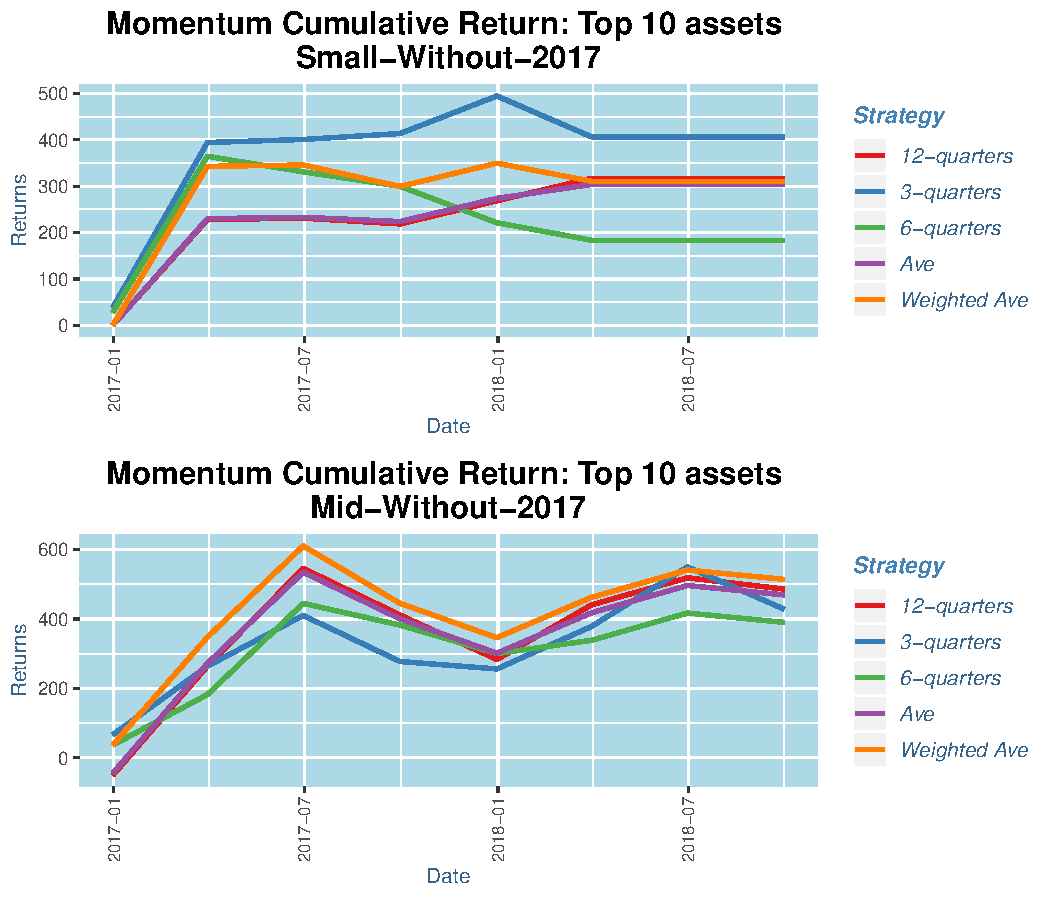
\includegraphics{IPA_Small_and_Mid_files/figure-latex/fig3-1.pdf}
\caption{\label{fig:OpdeltwithOut2017Q}Top 10 aktiver for Small- og Mid
cap uden transaktionsomkostninger med kvartalsvis rebalancering fra
2017}
\end{figure}

\rowcolors{2}{gray!6}{white}
\begin{table}

\caption{\label{tab:tab3}\label{tab:OpdeltwithOut2017Q}Top 10 aktiver for Small- og Mid cap uden transaktionsomkostninger med kvartalsvis rebalancering fra 2017}
\centering
\resizebox{\linewidth}{!}{
\begin{tabular}[t]{lrrrrrrrrrr}
\hiderowcolors
\toprule
\multicolumn{1}{c}{} & \multicolumn{5}{c}{Small cap} & \multicolumn{5}{c}{Mid cap} \\
\cmidrule(l{2pt}r{2pt}){2-6} \cmidrule(l{2pt}r{2pt}){7-11}
  & 3-quarters & 6-quarters & 12-quarters & Ave & Weighted Ave & 3-quarters & 6-quarters & 12-quarters & Ave & Weighted Ave\\
\midrule
\showrowcolors
Observations & 10.0000 & 10.0000 & 10.0000 & 10.0000 & 10.0000 & 8.0000 & 8.0000 & 8.0000 & 8.0000 & 8.0000\\
NAs & 3.0000 & 3.0000 & 3.0000 & 3.0000 & 3.0000 & 3.0000 & 3.0000 & 3.0000 & 3.0000 & 3.0000\\
Minimum & -88.1763 & -78.5792 & -12.5228 & -9.2785 & -46.2284 & -132.4685 & -81.6342 & -134.3574 & -134.3574 & -165.2003\\
Quartile 1 & 0.0000 & -32.9443 & 0.0000 & 0.0000 & -0.0900 & -46.5505 & -35.9701 & -69.6767 & -58.0000 & -45.0007\\
Median & 3.2933 & 0.0000 & 0.0000 & 0.0000 & 0.0000 & 94.3616 & 37.3377 & 22.6561 & 25.7711 & 57.8740\\
\addlinespace
Arithmetic Mean & 40.6361 & 18.3306 & 31.6870 & 30.3776 & 31.0593 & 53.5019 & 48.7585 & 60.7522 & 58.6644 & 64.2488\\
Geometric Mean & NaN & NaN & NaN & NaN & NaN & NaN & NaN & NaN & NaN & NaN\\
Quartile 3 & 31.8146 & 0.0000 & 36.9882 & 23.3055 & 2.2500 & 152.3029 & 95.3619 & 188.2883 & 152.8898 & 152.8898\\
Maximum & 356.0656 & 336.8378 & 228.1953 & 230.1006 & 342.8578 & 197.7456 & 262.5442 & 314.4812 & 316.4628 & 310.4428\\
SE Mean & 37.4537 & 36.6011 & 22.8602 & 22.9051 & 35.6004 & 46.1247 & 40.4034 & 62.3015 & 58.5204 & 58.4262\\
\addlinespace
LCL Mean (0.95) & -44.0900 & -64.4669 & -20.0263 & -21.4373 & -49.4744 & -55.5656 & -46.7804 & -86.5675 & -79.7144 & -73.9073\\
UCL Mean (0.95) & 125.3622 & 101.1282 & 83.4003 & 82.1925 & 111.5931 & 162.5694 & 144.2975 & 208.0719 & 197.0432 & 202.4049\\
Variance & 14027.7674 & 13396.4307 & 5225.8716 & 5246.4270 & 12673.9079 & 17019.8785 & 13059.5067 & 31051.8342 & 27397.1093 & 27308.9934\\
Stdev & 118.4389 & 115.7430 & 72.2902 & 72.4322 & 112.5785 & 130.4603 & 114.2782 & 176.2153 & 165.5207 & 165.2543\\
Skewness & 2.0431 & 2.3370 & 2.2724 & 2.3889 & 2.4086 & -0.4464 & 0.6822 & 0.3259 & 0.4373 & 0.1918\\
\addlinespace
Kurtosis & 3.3932 & 4.1566 & 3.7850 & 4.1702 & 4.3142 & -1.3675 & -0.4591 & -1.3836 & -1.1890 & -1.0787\\
NumberOfTrades & 91.0000 & 80.0000 & 105.0000 & 112.0000 & 114.0000 & 56.0000 & 46.0000 & 24.0000 & 30.0000 & 28.0000\\
\bottomrule
\end{tabular}}
\end{table}
\rowcolors{2}{white}{white}

Figur \ref{fig:OpdeltwithOut2017Q} viser nu et postivt afkast for begge
grupper. Tabel \ref{tab:OpdeltwithOut2017Q} giver værdier.

\hypertarget{kvartalsvis-rebalancering-med-transaktionsomkostninger}{%
\section{Kvartalsvis rebalancering med
transaktionsomkostninger}\label{kvartalsvis-rebalancering-med-transaktionsomkostninger}}

Det forsøges nu at implementere transaktionsomkostninger.

\begin{figure}
\centering
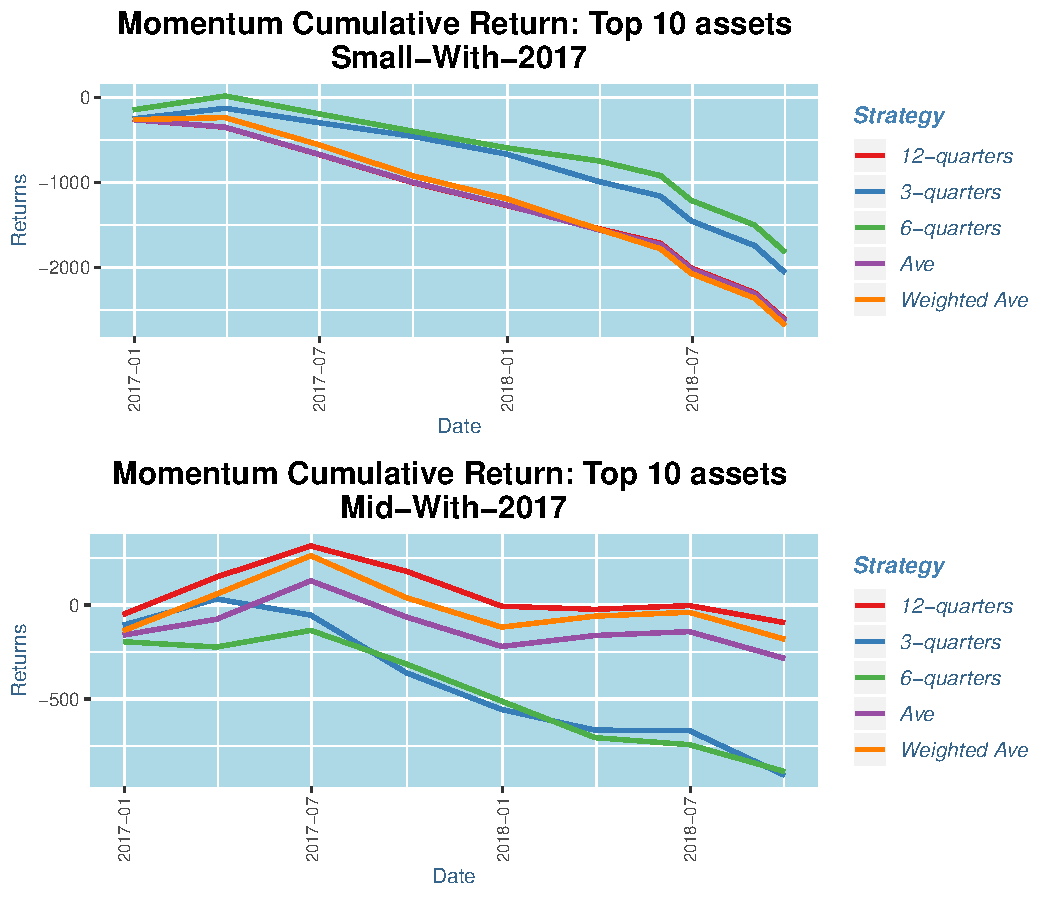
\includegraphics{IPA_Small_and_Mid_files/figure-latex/fig5-1.pdf}
\caption{\label{fig:Opdelt2017Q}Top 10 aktiver for Small- og Mid cap med
transaktionsomkostninger med kvartalsvis rebalancering fra 2017}
\end{figure}

\rowcolors{2}{gray!6}{white}
\begin{table}

\caption{\label{tab:tab5}\label{tab:Opdelt2017Q}Top 10 aktiver for Small- og Mid cap med transaktionsomkostninger med kvartalsvis rebalancering fra 2017}
\centering
\resizebox{\linewidth}{!}{
\begin{tabular}[t]{lrrrrrrrrrr}
\hiderowcolors
\toprule
\multicolumn{1}{c}{} & \multicolumn{5}{c}{Small cap} & \multicolumn{5}{c}{Mid cap} \\
\cmidrule(l{2pt}r{2pt}){2-6} \cmidrule(l{2pt}r{2pt}){7-11}
  & 3-quarters & 6-quarters & 12-quarters & Ave & Weighted Ave & 3-quarters & 6-quarters & 12-quarters & Ave & Weighted Ave\\
\midrule
\showrowcolors
Observations & 10.0000 & 10.0000 & 10.0000 & 10.0000 & 10.0000 & 8.0000 & 8.0000 & 8.0000 & 8.0000 & 8.0000\\
NAs & 3.0000 & 3.0000 & 3.0000 & 3.0000 & 3.0000 & 3.0000 & 3.0000 & 3.0000 & 3.0000 & 3.0000\\
Minimum & -320.1763 & -319.0000 & -331.5228 & -328.2785 & -365.2284 & -306.4685 & -197.6342 & -185.8226 & -192.3574 & -223.2003\\
Quartile 1 & -290.0000 & -269.3874 & -309.5000 & -309.5000 & -318.2500 & -206.0505 & -194.3507 & -101.5094 & -157.7151 & -146.5007\\
Median & -230.4938 & -199.8538 & -280.3412 & -289.4630 & -290.0000 & -108.6384 & -160.8802 & -33.5338 & -61.2289 & -58.1260\\
\addlinespace
Arithmetic Mean & -205.8639 & -181.7694 & -261.2130 & -262.5224 & -267.6407 & -113.2481 & -110.7415 & -11.7478 & -35.5856 & -22.7512\\
Geometric Mean & NaN & NaN & NaN & NaN & NaN & NaN & NaN & NaN & NaN & NaN\\
Quartile 3 & -169.0601 & -158.9220 & -263.0900 & -263.0900 & -263.0900 & -65.1971 & -35.1381 & 56.2721 & 64.8695 & 92.3645\\
Maximum & 124.0656 & 162.8378 & -90.8047 & -88.8994 & 23.8578 & 139.7456 & 88.5442 & 198.4812 & 204.5442 & 204.5442\\
SE Mean & 41.5666 & 42.7497 & 23.5082 & 23.7126 & 34.9500 & 49.4019 & 37.6023 & 48.1182 & 51.8335 & 58.6972\\
\addlinespace
LCL Mean (0.95) & -299.8942 & -278.4759 & -314.3922 & -316.1639 & -346.7031 & -230.0649 & -199.6568 & -125.5294 & -158.1524 & -161.5480\\
UCL Mean (0.95) & -111.8336 & -85.0628 & -208.0337 & -208.8808 & -188.5783 & 3.5688 & -21.8261 & 102.0338 & 86.9812 & 116.0456\\
Variance & 17277.8584 & 18275.3612 & 5526.3566 & 5622.8571 & 12215.0288 & 19524.3587 & 11311.4748 & 18522.9222 & 21493.7199 & 27562.8853\\
Stdev & 131.4453 & 135.1864 & 74.3395 & 74.9857 & 110.5216 & 139.7296 & 106.3554 & 136.0989 & 146.6074 & 166.0207\\
Skewness & 1.6432 & 1.6990 & 1.3849 & 1.4583 & 1.9848 & 0.4402 & 0.8483 & 0.4376 & 0.3762 & 0.2974\\
\addlinespace
Kurtosis & 2.0849 & 2.4465 & 0.8285 & 0.9392 & 3.1161 & -0.4609 & -0.6637 & -1.0368 & -1.2978 & -1.4403\\
NumberOfTrades & 91.0000 & 80.0000 & 105.0000 & 112.0000 & 114.0000 & 56.0000 & 46.0000 & 24.0000 & 30.0000 & 28.0000\\
\bottomrule
\end{tabular}}
\end{table}
\rowcolors{2}{white}{white}

Figur \ref{fig:Opdelt2017Q} viser, at med implementeringen af
transaktionsomkostninger vil der være et tab. Tabel
\ref{tab:Opdelt2017Q} giver værdier.

\hypertarget{kvartalsvis-rebalancering-med-transaktionsomkostninger-med-get-handel}{%
\section{Kvartalsvis rebalancering med transaktionsomkostninger med øget
handel}\label{kvartalsvis-rebalancering-med-transaktionsomkostninger-med-get-handel}}

For at mindske effekten af transaktionsomkostninger forsøges nu at
handle med 15 aktiver pr. gang i stedet for blot en. Dette vil for de
fleste aktiver stadig holde dem under minimumsgrænsen på 29 kr.

\begin{figure}
\centering
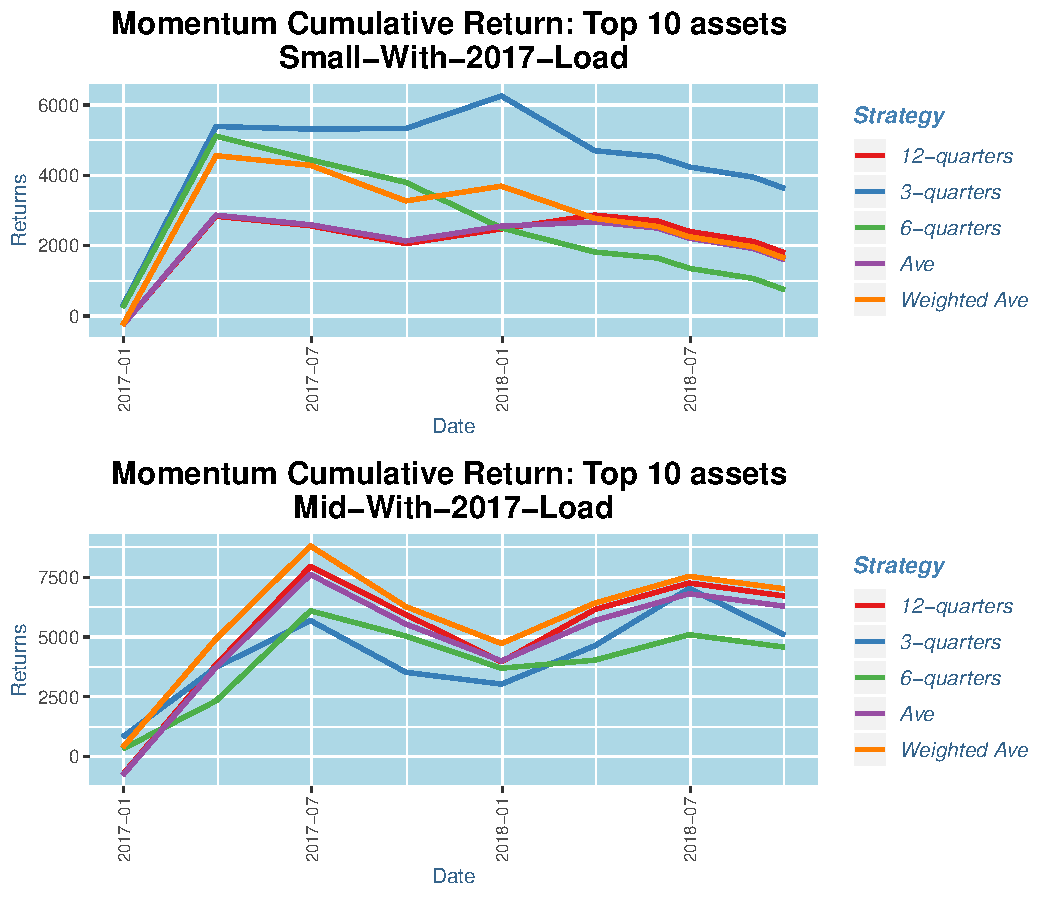
\includegraphics{IPA_Small_and_Mid_files/figure-latex/fig6-1.pdf}
\caption{\label{fig:Opdelt2017QLoad}Top 10 aktiver for Small- og Mid cap
med transaktionsomkostninger med kvartalsvis rebalancering fra 2017 med
øget handel}
\end{figure}

\rowcolors{2}{gray!6}{white}
\begin{table}

\caption{\label{tab:tab6}\label{tab:Opdelt2017QLoad}Top 10 aktiver for Small- og Mid cap med transaktionsomkostninger med kvartalsvis rebalancering fra 2017 med øget handel}
\centering
\resizebox{\linewidth}{!}{
\begin{tabular}[t]{lrrrrrrrrrr}
\hiderowcolors
\toprule
\multicolumn{1}{c}{} & \multicolumn{5}{c}{Small cap} & \multicolumn{5}{c}{Mid cap} \\
\cmidrule(l{2pt}r{2pt}){2-6} \cmidrule(l{2pt}r{2pt}){7-11}
  & 3-quarters & 6-quarters & 12-quarters & Ave & Weighted Ave & 3-quarters & 6-quarters & 12-quarters & Ave & Weighted Ave\\
\midrule
\showrowcolors
Observations & 10.0000 & 10.0000 & 10.0000 & 10.0000 & 10.0000 & 8.0000 & 8.0000 & 8.0000 & 8.0000 & 8.0000\\
NAs & 3.0000 & 3.0000 & 3.0000 & 3.0000 & 3.0000 & 3.0000 & 3.0000 & 3.0000 & 3.0000 & 3.0000\\
Minimum & -320.1763 & -319.0000 & -331.5228 & -328.2785 & -365.2284 & -306.4685 & -197.6342 & -185.8226 & -192.3574 & -223.2003\\
Quartile 1 & -290.0000 & -269.3874 & -309.5000 & -309.5000 & -318.2500 & -206.0505 & -194.3507 & -101.5094 & -157.7151 & -146.5007\\
Median & -230.4938 & -199.8538 & -280.3412 & -289.4630 & -290.0000 & -108.6384 & -160.8802 & -33.5338 & -61.2289 & -58.1260\\
\addlinespace
Arithmetic Mean & -205.8639 & -181.7694 & -261.2130 & -262.5224 & -267.6407 & -113.2481 & -110.7415 & -11.7478 & -35.5856 & -22.7512\\
Geometric Mean & NaN & NaN & NaN & NaN & NaN & NaN & NaN & NaN & NaN & NaN\\
Quartile 3 & -169.0601 & -158.9220 & -263.0900 & -263.0900 & -263.0900 & -65.1971 & -35.1381 & 56.2721 & 64.8695 & 92.3645\\
Maximum & 124.0656 & 162.8378 & -90.8047 & -88.8994 & 23.8578 & 139.7456 & 88.5442 & 198.4812 & 204.5442 & 204.5442\\
SE Mean & 41.5666 & 42.7497 & 23.5082 & 23.7126 & 34.9500 & 49.4019 & 37.6023 & 48.1182 & 51.8335 & 58.6972\\
\addlinespace
LCL Mean (0.95) & -299.8942 & -278.4759 & -314.3922 & -316.1639 & -346.7031 & -230.0649 & -199.6568 & -125.5294 & -158.1524 & -161.5480\\
UCL Mean (0.95) & -111.8336 & -85.0628 & -208.0337 & -208.8808 & -188.5783 & 3.5688 & -21.8261 & 102.0338 & 86.9812 & 116.0456\\
Variance & 17277.8584 & 18275.3612 & 5526.3566 & 5622.8571 & 12215.0288 & 19524.3587 & 11311.4748 & 18522.9222 & 21493.7199 & 27562.8853\\
Stdev & 131.4453 & 135.1864 & 74.3395 & 74.9857 & 110.5216 & 139.7296 & 106.3554 & 136.0989 & 146.6074 & 166.0207\\
Skewness & 1.6432 & 1.6990 & 1.3849 & 1.4583 & 1.9848 & 0.4402 & 0.8483 & 0.4376 & 0.3762 & 0.2974\\
\addlinespace
Kurtosis & 2.0849 & 2.4465 & 0.8285 & 0.9392 & 3.1161 & -0.4609 & -0.6637 & -1.0368 & -1.2978 & -1.4403\\
NumberOfTrades & 91.0000 & 80.0000 & 105.0000 & 112.0000 & 114.0000 & 56.0000 & 46.0000 & 24.0000 & 30.0000 & 28.0000\\
\bottomrule
\end{tabular}}
\end{table}
\rowcolors{2}{white}{white}

Figur \ref{fig:Opdelt2017QLoad} viser nu igen positiv afkast. Dvs. ved
at øge antallet af aktiver pr. handel, da vil man mindske effekten af
transafktionsomkostninger set i \ref{fig:Opdelt2017Q} og få effekt af
den trend man så i figur \ref{fig:OpdeltwithOut2017Q}. Tabel
\ref{tab:Opdelt2017QLoad} giver værdier.

\hypertarget{error-adjusted-momentum}{%
\section{Error adjusted momentum}\label{error-adjusted-momentum}}

En anden måde at mindske effekten af transaktionsomkostninger er at
mindske antallet af handler. Derfor forsøges nu med en mere robust
strategi ``Error Adjusted'' relativ momentum. I stedet for at rangere
aktiverne på baggrund af ROC, da gør man det på bagkant af ROC divideret
med et fejlled. Man laver en forudsigelse af næste dags ROC ved en
simpel moving average af de sidste 10 dages ROC. Herefter finder man
fejlledet af ROC og forudsigelsen, og laver så igen en simpel moving
average igen på de seneste 10 dage af dette fejlled. Til sidst divideres
ROC med dette fejlled for at justere afkastene med volatilitet. Hvis
aktivet oplever stor votalitet, da ønsker man at tillægge disse perioder
mindre værdi, da de er mere usikre. Fejlledene vil i disse perioder være
større, hvorved ROC vil blive justeret og blive mindre. Dette kan gøre,
at hvis der er nogle aktiver, som ligger og skifter mellem om man skal
have en position i den ene eller den anden, da vil man kunne opnå en
mere stabil sammenligning.

\begin{figure}
\centering
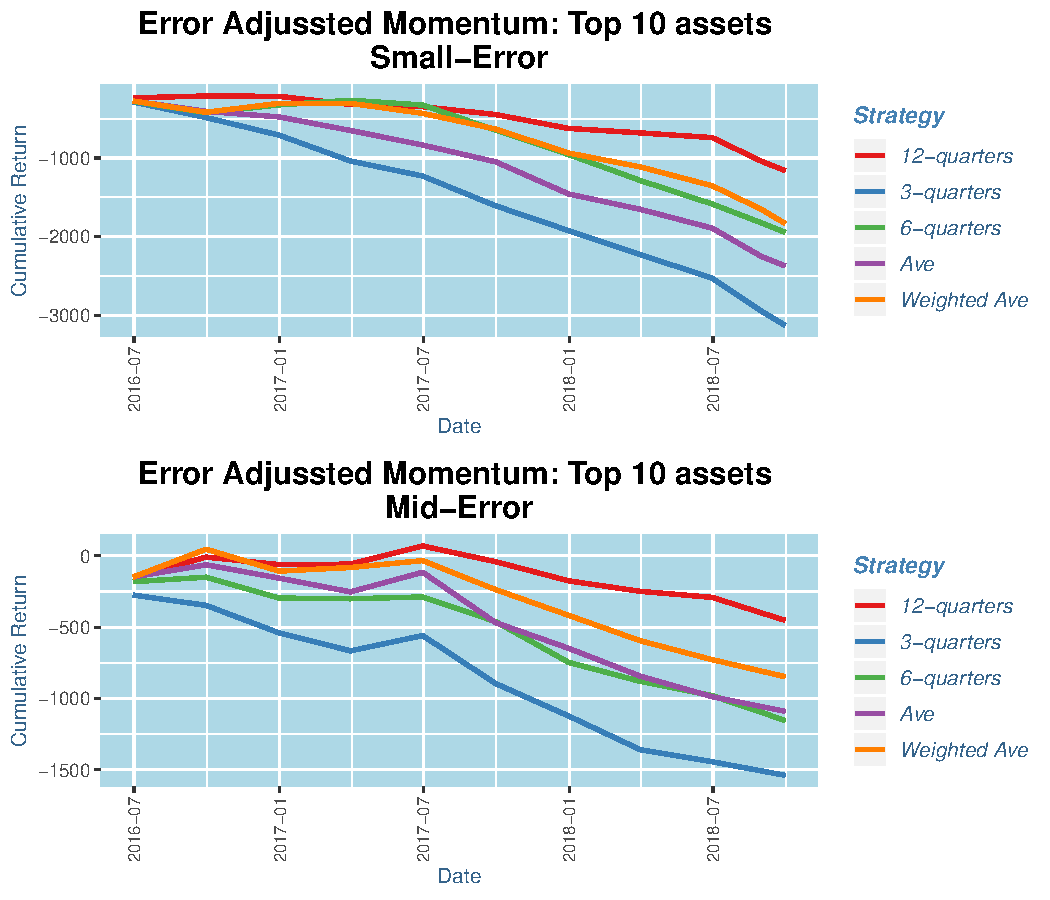
\includegraphics{IPA_Small_and_Mid_files/figure-latex/fig7-1.pdf}
\caption{\label{fig:Opdelt2017QErr}Top 10 aktiver for Small- og Mid cap
med transaktionsomkostninger med kvartalsvis rebalancering fra 2017 med
Error adjustedmomentum}
\end{figure}

\rowcolors{2}{gray!6}{white}
\begin{table}

\caption{\label{tab:tab7}\label{tab:Opdelt2017QErr}Top 10 aktiver for Small- og Mid cap med transaktionsomkostninger med kvartalsvis rebalancering fra 2017 med Error adjustedmomentum}
\centering
\resizebox{\linewidth}{!}{
\begin{tabular}[t]{lrrrrrrrrrr}
\hiderowcolors
\toprule
\multicolumn{1}{c}{} & \multicolumn{5}{c}{Small cap} & \multicolumn{5}{c}{Mid cap} \\
\cmidrule(l{2pt}r{2pt}){2-6} \cmidrule(l{2pt}r{2pt}){7-11}
  & 3-quarters & 6-quarters & 12-quarters & Ave & Weighted Ave & 3-quarters & 6-quarters & 12-quarters & Ave & Weighted Ave\\
\midrule
\showrowcolors
Observations & 11.0000 & 11.0000 & 11.0000 & 11.0000 & 11.0000 & 10.0000 & 10.0000 & 10.0000 & 10.0000 & 10.0000\\
NAs & 1.0000 & 1.0000 & 1.0000 & 1.0000 & 1.0000 & 1.0000 & 1.0000 & 1.0000 & 1.0000 & 1.0000\\
Minimum & -420.0000 & -328.9500 & -300.2000 & -409.0700 & -304.5400 & -336.2731 & -285.9047 & -160.8898 & -352.7004 & -203.3710\\
Quartile 1 & -322.1792 & -304.8250 & -148.4340 & -258.2545 & -258.2545 & -233.6522 & -173.7420 & -128.0373 & -172.3126 & -171.8981\\
Median & -300.0000 & -240.0000 & -98.9809 & -194.2887 & -180.0000 & -159.3856 & -139.5018 & -63.1076 & -123.7810 & -140.7317\\
\addlinespace
Arithmetic Mean & -284.4090 & -176.9422 & -105.6569 & -215.7265 & -166.7327 & -153.8387 & -115.4004 & -45.1904 & -108.9946 & -84.6929\\
Geometric Mean & NaN & NaN & NaN & NaN & NaN & NaN & NaN & NaN & NaN & NaN\\
Quartile 3 & -211.1906 & -90.7295 & -42.8936 & -152.3115 & -135.6267 & -87.6392 & -29.1311 & -8.2329 & -94.3229 & -10.7096\\
Maximum & -180.0000 & 99.2302 & 23.2460 & -70.7105 & 114.2757 & 107.1713 & 31.7959 & 141.2231 & 137.2897 & 195.3659\\
SE Mean & 23.6204 & 46.7933 & 29.7610 & 30.5947 & 38.6236 & 40.1473 & 31.9491 & 34.0229 & 43.9534 & 41.1715\\
\addlinespace
LCL Mean (0.95) & -337.0385 & -281.2041 & -171.9686 & -283.8957 & -252.7913 & -244.6582 & -187.6742 & -122.1556 & -208.4242 & -177.8292\\
UCL Mean (0.95) & -231.7795 & -72.6803 & -39.3453 & -147.5573 & -80.6740 & -63.0191 & -43.1266 & 31.7748 & -9.5651 & 8.4434\\
Variance & 6137.1460 & 24085.7303 & 9742.8805 & 10296.3863 & 16409.5726 & 16118.0730 & 10207.4235 & 11575.5937 & 19319.0223 & 16950.8879\\
Stdev & 78.3399 & 155.1958 & 98.7060 & 101.4711 & 128.0999 & 126.9570 & 101.0318 & 107.5899 & 138.9929 & 130.1956\\
Skewness & -0.1401 & 0.6736 & -0.6681 & -0.5857 & 1.0029 & 0.5746 & 0.1110 & 0.7557 & 0.2973 & 1.1442\\
\addlinespace
Kurtosis & -1.0098 & -0.9631 & -0.4799 & -0.4840 & 0.2065 & -0.0950 & -0.8960 & -0.7158 & -0.1079 & 0.0145\\
NumberOfTrades & 110.0000 & 78.0000 & 46.0000 & 84.0000 & 74.0000 & 62.0000 & 56.0000 & 36.0000 & 56.0000 & 46.0000\\
\bottomrule
\end{tabular}}
\end{table}
\rowcolors{2}{white}{white}

Figur \ref{fig:Opdelt2017QErr} viser at også Error adjusted momentum
ikke ``overlever'' transactionsomkostninger. Man kan se i Tabbel
\ref{tab:Opdelt2017QErr}, at for Small cap, bortsetframomentum på 3
måneder, da er antallet af handler mindre sammenlignet med tabel
\ref{tab:Opdelt2017Q}. For Mid cap er antallet af handler større for
samtlige strategier. Det virker derfor ikke til, at man ved en Erro
Adjustment kan nedbringe antallet af handlet i dette tilfælde.

\hypertarget{error-adjusted-momentum-med-loading}{%
\section{Error adjusted momentum med
loading}\label{error-adjusted-momentum-med-loading}}

Det forsøges nu at se, om man ved load igen kan skabe en positiv profit.

\begin{figure}
\centering
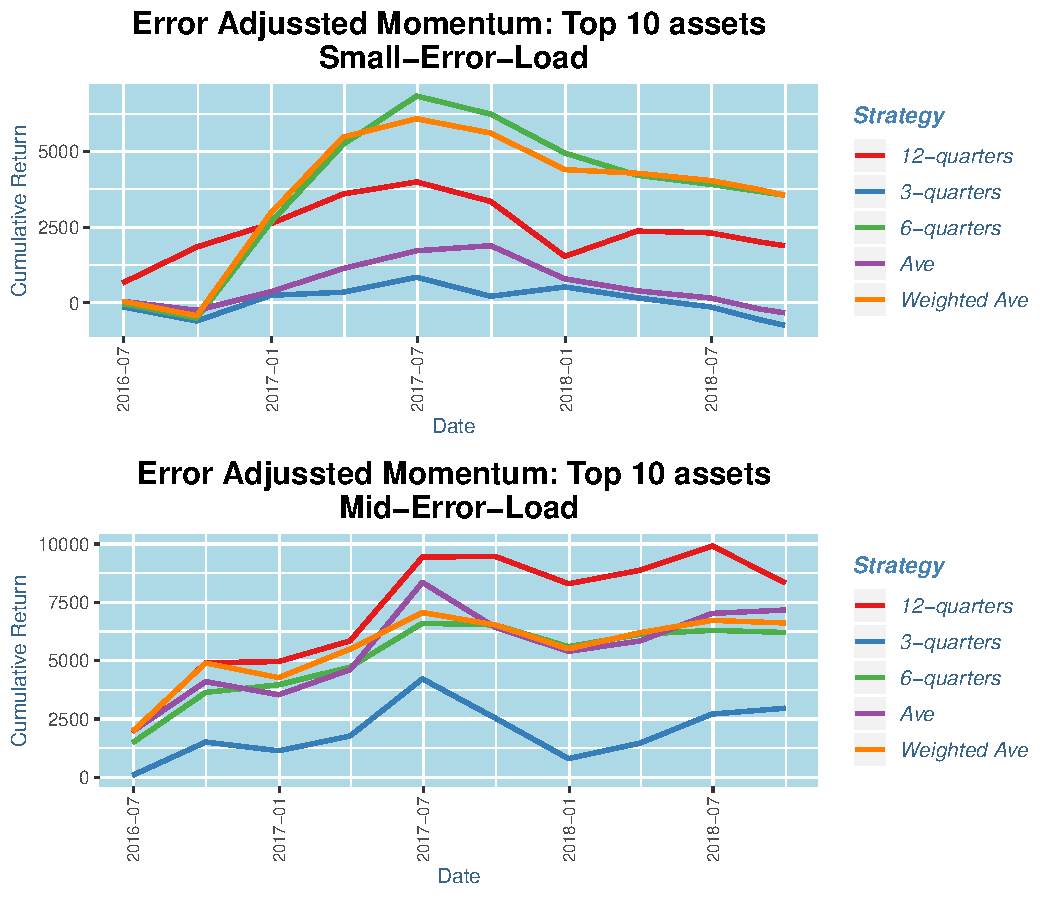
\includegraphics{IPA_Small_and_Mid_files/figure-latex/fig8-1.pdf}
\caption{\label{fig:Opdelt2017QErrLoad}Top 10 aktiver for Small- og Mid
cap med transaktionsomkostninger med kvartalsvis rebalancering fra 2017
med Error adjustedmomentum og loading}
\end{figure}

\rowcolors{2}{gray!6}{white}
\begin{table}

\caption{\label{tab:tab8}\label{tab:Opdelt2017QErrLoad}Top 10 aktiver for Small- og Mid cap med transaktionsomkostninger med kvartalsvis rebalancering fra 2017 med Error adjustedmomentum  og loading}
\centering
\resizebox{\linewidth}{!}{
\begin{tabular}[t]{lrrrrrrrrrr}
\hiderowcolors
\toprule
\multicolumn{1}{c}{} & \multicolumn{5}{c}{Small cap} & \multicolumn{5}{c}{Mid cap} \\
\cmidrule(l{2pt}r{2pt}){2-6} \cmidrule(l{2pt}r{2pt}){7-11}
  & 3-quarters & 6-quarters & 12-quarters & Ave & Weighted Ave & 3-quarters & 6-quarters & 12-quarters & Ave & Weighted Ave\\
\midrule
\showrowcolors
Observations & 11.0000 & 11.0000 & 11.0000 & 11.0000 & 11.0000 & 10.0000 & 10.0000 & 10.0000 & 10.0000 & 10.0000\\
NAs & 1.0000 & 1.0000 & 1.0000 & 1.0000 & 1.0000 & 1.0000 & 1.0000 & 1.0000 & 1.0000 & 1.0000\\
Minimum & -630.1500 & -1284.7500 & -1813.0192 & -1096.0500 & -1208.1000 & -1732.0573 & -928.5700 & -1573.3465 & -1930.5054 & -1023.0117\\
Quartile 1 & -394.5651 & -538.0387 & -211.5000 & -333.4249 & -388.9500 & -259.9098 & -11.1794 & 32.2275 & -388.4525 & -425.8234\\
Median & -180.0000 & -240.0000 & 398.9475 & -120.0000 & -180.0000 & 443.1342 & 427.4726 & 732.0860 & 760.0691 & 609.1932\\
\addlinespace
Arithmetic Mean & -67.5326 & 322.9061 & 171.5096 & -29.9418 & 322.9374 & 296.4197 & 620.9941 & 834.1443 & 717.0804 & 661.6071\\
Geometric Mean & NaN & NaN & NaN & NaN & NaN & NaN & NaN & NaN & NaN & NaN\\
Quartile 3 & 207.3117 & 784.5673 & 803.0837 & 376.5761 & 326.1899 & 1098.4515 & 1302.5646 & 1725.0478 & 1773.5017 & 1479.3676\\
Maximum & 847.3365 & 3168.4536 & 1188.6901 & 768.2097 & 3394.1361 & 2447.5697 & 2156.9385 & 3590.3342 & 3739.3449 & 2930.4885\\
SE Mean & 137.8053 & 436.8000 & 265.2571 & 164.6874 & 417.1511 & 416.1543 & 305.1402 & 522.2809 & 528.5906 & 401.7252\\
\addlinespace
LCL Mean (0.95) & -374.5819 & -650.3449 & -419.5200 & -396.8881 & -606.5331 & -644.9866 & -69.2809 & -347.3372 & -478.6746 & -247.1585\\
UCL Mean (0.95) & 239.5167 & 1296.1571 & 762.5392 & 337.0046 & 1252.4079 & 1237.8261 & 1311.2692 & 2015.6259 & 1912.8355 & 1570.3728\\
Variance & 208893.2426 & 2098736.3125 & 773974.4915 & 298341.2853 & 1914165.1894 & 1731843.7383 & 931105.3140 & 2727773.7313 & 2794080.5960 & 1613831.7119\\
Stdev & 457.0484 & 1448.7016 & 879.7582 & 546.2063 & 1383.5336 & 1315.9953 & 964.9380 & 1651.5973 & 1671.5504 & 1270.3668\\
Skewness & 0.7397 & 1.0097 & -0.9693 & -0.2011 & 1.3535 & -0.2102 & 0.2225 & 0.2316 & 0.1609 & 0.3291\\
\addlinespace
Kurtosis & -0.5426 & -0.4266 & 0.2853 & -0.4648 & 0.5575 & -0.6782 & -0.8794 & -0.8405 & -0.6103 & -0.9439\\
NumberOfTrades & 110.0000 & 78.0000 & 46.0000 & 84.0000 & 74.0000 & 62.0000 & 56.0000 & 36.0000 & 56.0000 & 46.0000\\
\bottomrule
\end{tabular}}
\end{table}
\rowcolors{2}{white}{white}

Figur \ref{fig:Opdelt2017QErrLoad} viser igen, at man ved et load kan
opnå trend på markdet. Tabel \ref{tab:Opdelt2017QErrLoad} giver værdier.

\hypertarget{konklusion}{%
\section{Konklusion}\label{konklusion}}

Analysen har forsøgt at se på om man kan finde en trend på det danske
Small- og Mid cap marked, og om man ved momentum strategier kan opnå en
profit. Momentum er i høj grad påvirket af hvilket regime markedet
befinder sig i og fra 2017 til i dag er der ingen af de undersøgte
strategier, der giver positivt afkast med månedlige rebalanceringer.
Hvis man i steder rebalancerer kvartalsvis vil man kunne se en positiv
trend.\\
Tager man herefter højde for markedsomkostninger, da vil man ved en
strategi, hvor man kun handler et aktiv pr gang, blive ``spist'' op ad
handelsomkostninger. Man må derfor handle flere aktiver pr. handel. Gør
man dette vil man kunne få del i den positive trend og modvirke den
negative effekt handelsomkostninger har.

Til videre arbejde kan man se på hvilken strategi der optimere afkast.
Der kan dog tvivles på resultatet af dette, da momentum er meget
afhængigt af hvilken tidsperiode, der kigges over, og en optimal
strategi for alle perider virker usandsynlig.\\
Videre arbejde kunne også væreen implementering i at gå ``cash'', hvis
samtlige aktiver viser dårlig trend.


\end{document}
